%
% kreis.tex
%
% (c) 2021 Prof Dr Andreas Müller, OST Ostschweizer Fachhochschule
%
\section{Kreisförmige Membran
\label{buch:pde:section:kreis}}
\rhead{Kreisförmige Membran}
In diesem Abschnitt soll die Differentialgleichung einer kreisförmigen
Membran mit Hilfe der Separationsmethode gelöst werden.
Dabei werden die Bessel-Funktionen als Lösungsfunktionen 
auftreten und die Eigenfrequenzen werden durch ihre Nullstellen
berechnet.

\subsection{Differentialgleichung und Randbedingung}
Die Wellengleichung auf einem Kreisgebiet mit Radius $r_0$ 
lässt sich am besten mit Hilfe von Polarkoordinaten $(r,\varphi)$
ausdrücken.
Gesucht ist also eine Funktion $u(t,r,\varphi)$ gesucht, wobei
$0\le r<r_0$ und $0\le \varphi\le 2\pi$.
Die Funktion muss eine Lösung der Wellengleichung
\[
\frac{1}{c^2}\frac{\partial^2u}{\partial t^2} = \Delta u
\]
sein.

Der Laplace-Operator hat in Polarkoordinaten die Form
\begin{equation}
\Delta
=
\frac{\partial^2}{\partial r^2}
+
\frac1r
\frac{\partial}{\partial r}
+
\frac{1}{r^2}
\frac{\partial^2}{\partial\varphi^2}.
\label{buch:pde:kreis:laplace}
\end{equation}
Die Differentialgleichung ist 
\[
\frac{1}{c^2} \frac{\partial^2 u}{\partial t^2}
=
\Delta u.
\]
Die Separation der Zeit führt auf die Eigenwertgleichung
\[
\Delta U(r,\varphi) = -\lambda^2 U(r,\varphi)
\]
für eine Funktion, die nur von $r$ und $\varphi$ abhängt.

Die Randbedingungen besagen, dass $u(t,r_0,\varphi)=0$ für $t>0$.
Dies bedeutet für die Funktion $U(r,\varphi)$, dass
$U(r_0,\varphi)=0$ sein muss für alle $\varphi$.

Die Bedingungen an $U$ reichen aber nicht ganz.
Alle Koordinaten $(0,\varphi)$ bezeichnen ja gleichermassen
den Nullpunkt des Koordinatensystems, es muss also auch sichergestellt
sein, dass $U(0,\varphi)$ für alle $\varphi$ den gleichen Wert gibt.

\subsection{Separation}
Das Eigenwertproblem $\Delta U=-\lambda^2 U$ soll jetzt in Polarkoordinaten
separiert werden.
Dazu schreiben wir die Lösung als
\[
U(r,\varphi)
=
R(r)\cdot \Phi(\varphi).
\]
Die Randbedingungen an $U$ werden zu $R(r_0)=0$.

Im Ursprung des Koordinatensystems ist die Randbedingung etwas
komplizierter.
Wenn $R(0)=0$ ist, dann ist sichergestellt, dass
$U(0,\varphi)=R(0)\Phi(\varphi)0$ ist, dass also der Wert unabhängig
ist von $\varphi$.
Wenn aber $R(0)\ne 0$ ist, dann kann die geforderte Unabhängigkeit
von $\varphi$ nur erfüllt werden, wenn $\Phi(\varphi)$ konstant ist.
Da die Funktion aber auch noch differenzierbar sein soll, darf es
an der Stelle $r=0$ keine ``Spitze'' geben, die Ableitung $R'(0)$
muss also auch $=0$ sein.
% XXX Evtl Bild zur Illustration dieses Problems

Die Differntialgleichungen wird mit der Form~\eqref{buch:pde:kreis:laplace}
des Laplace-Operators
\[
\Delta U
=
R''(r) \Phi(\varphi)
+
\frac1r R'(r)\Phi(\varphi)
+
\frac{1}{r^2} R(r)\Phi''(\varphi)
=
-\lambda^2
R(r)\Phi(\varphi)
\]
Nach Division durch die rechte Seite erhalten wir
\[
\frac{R''(r)}{R(r)}
+
\frac1r \frac{R'(r)}{R(r)}
+
\frac{1}{r^2} \frac{\Phi''(\varphi)}{\Phi(\varphi)}
=
-\lambda^2
\]
Im letzten Term auf der linken Seite kommen die Variablen $r$ und $\varphi$
gemischt vor, man muss also die Gleichung erst mit $r^2$ multiplizieren,
bevor man sie in 
\[
\frac{r^2R''(r)+rR'(r)+\lambda^2 r^2R(r)}{R(r)}
=
-\frac{\Phi''(\varphi)}{\Phi(\varphi)}
\]
separieren kann.
Die beiden Seiten sind also konstant, wir nennen die gemeinsame
Konstanten $\mu^2$, das vereinfacht die Lösung der Gleichung
für $\Phi(\varphi)$.

Die Gleichung für $\Phi$ hat für $\mu\ne 0$ die Lösungen
\begin{align*}
\Phi(\varphi) &= \cos\mu\varphi
&&\text{und}&
\Phi(\varphi) &= \sin\mu\varphi.
\end{align*}
Die Lösung muss aber auch stetig sein, d.~h.~es muss $\Phi(0)=\Phi(2\pi)$
gelten.
Dies ist nur möglich, wenn $\mu$ eine ganze Zahl ist.

Für $\mu=0$ hat das charakteristische Polynome eine doppelte Nullstelle,
die allgemeine Lösung lautet daher
\[
\Phi(\varphi)= C \varphi + D.
\]
Die Funktion $\Phi$ muss aber auch stetig sein, d.~h.~$\Phi(0)=\Phi(2\pi)$,
das ist mit $C\ne 0$ nicht möglich, somit kommt für $\mu=0$ nur die
Lösung $\Phi(\varphi)=D$ in Frage.

Die Gleichung für $R(r)$ wird jetzt
\begin{equation}
r^2R''(r) + rR'(r)+(\lambda^2 r^2-\mu^2)R(r)
=
0.
\label{buch:pde:kreis:Rdgl}
\end{equation}
Bis auf den Faktor $\lambda^2$ ist dies eine Besselsche Differentialgleichung.

\subsection{Umformung in eine Besselsche Differentialgleichung}
Die Funktion $y(x) = J_\mu(sx)$ hat die Ableitungen
\begin{align*}
y'(x) &= sJ'_mu(sx)      
\\
y''(x) &= s^2J''_\mu(sx)
\end{align*}
Setzt man dies in die Besselsche Differentialgleichung für $J_\mu$ an
der Stelle $sx$ ein, erhält man
\[
s^2x^2 J''_\mu(sx) + sx J'_\mu(sx) + (s^2x^2 -\mu^2) J_\mu(sx) = 0.
\]
Die Differentialgleichung \eqref{buch:pde:kreis:Rdgl} der Funktion $R(r)$
wird also gelöst von den Funktionen $R(r) = J_\mu(\lambda r)$.

\subsection{Eigenfrequenzen}
Im vorangegangenen Abschnitt haben wir gefunden, dass die Lösungen
für $R(r)$ die Funktionen $J_\mu(\lambda r)$ sind.
Bis jetzt haben wir aber nicht nachgeprüft, dass die Randbedingung
eingehalten wird. 
Diese ist erfüllt, $R(r_0)=0$ ist.
Es muss also
$J_\mu(\lambda r_0)=0$ sein, oder $\lambda r_0$ muss eine
Nullstelle von $J_{\mu}$ sein.
Bezeichnen wir die Nullstellen von $J_\mu$ mit $j_{\mu k}$, wobei $k$
eine natürliche Zahl ist, dann muss
\[
\lambda = \frac{j_{\mu k}}{r_0}
\]
sein.
Die Eigenfrequenzen der kreisförmigen Membran werden also im Wesentlichen
durch die Nullstellen der Bessel-Funktionen gegeben.

Zu jedem ganzzahligen $\mu$ gibt es also eine Folge $j_{\mu k}/r_0$  von
Eigenfrequenzen. 
Die Lösungen mit Index $k$ der Differentialgleichung mit Index $k$ hat
die Form
\[
U_{\mu k}(r,\varphi)
=
C \cos(\mu \varphi+\delta)
J_{\mu}\biggl(
\frac{j_{\mu k}}{r_0}r
\biggr)
\]
Der Faktor $J_{\mu}$ hat $k$ weitere Nullstellen für Radien $r<r_0$,diese
gehören zu kreisförmigen Knotenlinien der Membran, dort bewegt sie sich
nicht.
Der Faktor $\cos(\mu\varphi+\delta)$ hat $2\mu$ Nullstellen im Intervall
$[0,2\pi)$, es gibt also noch zusätzlich $\mu$ diametrale Knotenlinien.
Nur für $\mu=0$ gibt es Lösungen, die keine radialen Knotenlinien haben,
da in diesem Fall $\Phi$ eine konstante Funktion sein muss.

\begin{table}
\centering
\begin{tabular}{|>{$}c<{$}|>{$}r<{$}|>{$}r<{$}|>{$}r<{$}|>{$}r<{$}|>{$}r<{$}|>{$}r<{$}|>{$}r<{$}|>{$}r<{$}|}
\hline
 k & \mu = 0 & \mu = 1 & \mu = 2 & \mu = 3 & \mu = 4 & \mu = 5 & \mu = 6 & \mu = 7 \\
\hline
 0 &   2.4048& 0\phantom{.0000}& 0\phantom{.0000}& 0\phantom{.0000}& 0\phantom{.0000}& 0\phantom{.0000}& 0\phantom{.0000}& 0\phantom{.0000}\\
 1 &   5.5201&   3.8317&   5.1356&   6.3802&   7.5883&   8.7715&   9.9361&  11.0864\\
 2 &   8.6537&   7.0156&   8.4172&   9.7610&  11.0647&  12.3386&  13.5893&  14.8213\\
 3 &  11.7915&  10.1735&  11.6198&  13.0152&  14.3725&  15.7002&  17.0038&  18.2876\\
 4 &  14.9309&  13.3237&  14.7960&  16.2235&  17.6160&  18.9801&  20.3208&  21.6415\\
 5 &  18.0711&  16.4706&  17.9598&  19.4094&  20.8269&  22.2178&  23.5861&  24.9349\\
 6 &  21.2116&  19.6159&  21.1170&  22.5827&  24.0190&  25.4303&  26.8202&  28.1912\\
 7 &  24.3525&  22.7601&  24.2701&  25.7482&  27.1991&  28.6266&  30.0337&  31.4228\\
 8 &  27.4935&  25.9037&  27.4206&  28.9084&  30.3710&  31.8117&  33.2330&  34.6371\\
 9 &  30.6346&  29.0468&  30.5692&  32.0649&  33.5371&  34.9888&  36.4220&  37.8387\\
 10 &  33.7758&  32.1897&  33.7165&  35.2187&  36.6990&  38.1599&  39.6032&  41.0308\\
\hline
\end{tabular}

\caption{Nullstellen der Bessel-Funktionen
\label{buch:pde:kreis:table:besselzeros}}
\end{table}

\begin{figure}
\centering
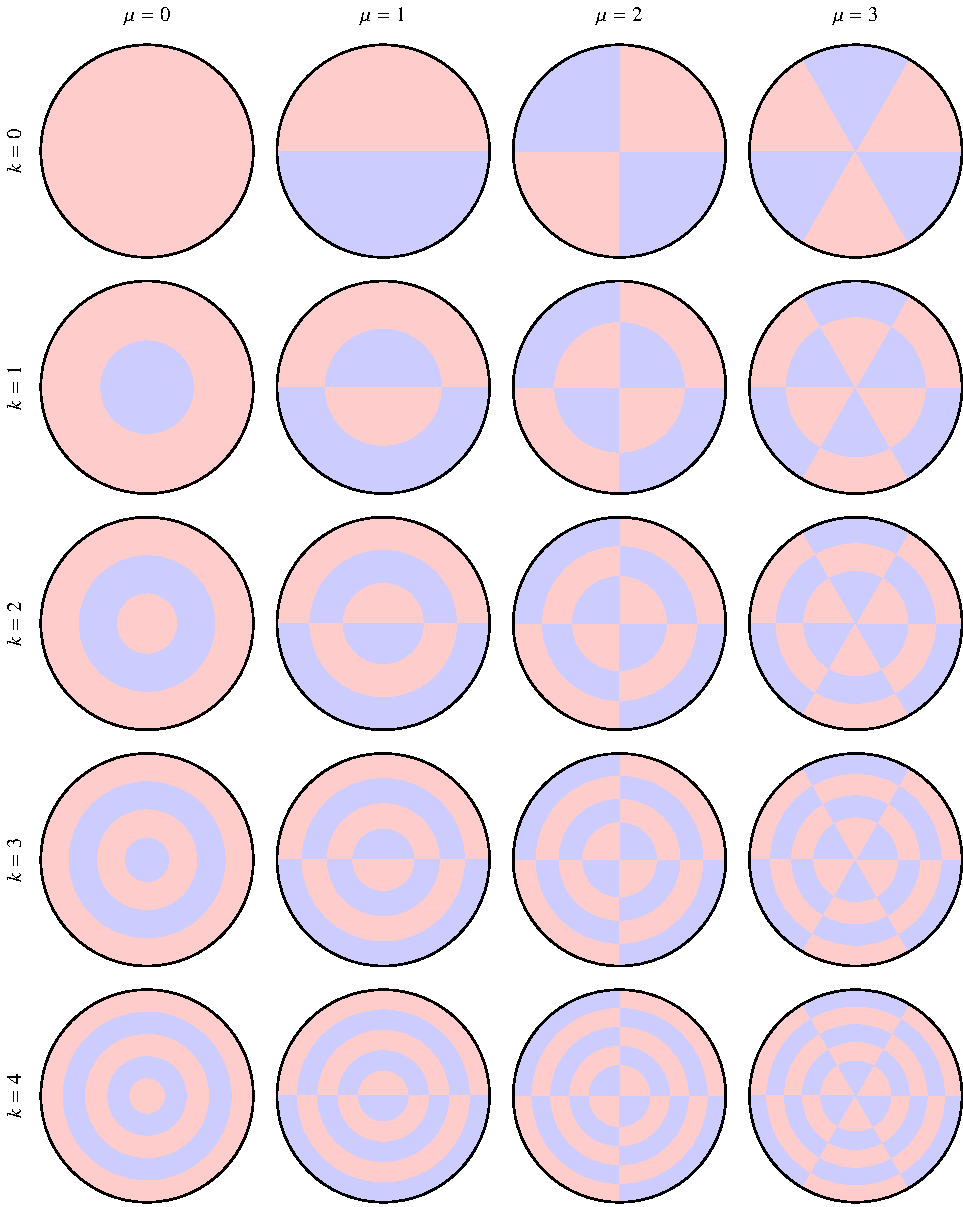
\includegraphics[width=\textwidth]{chapters/090-pde/bessel/pauke.pdf}
%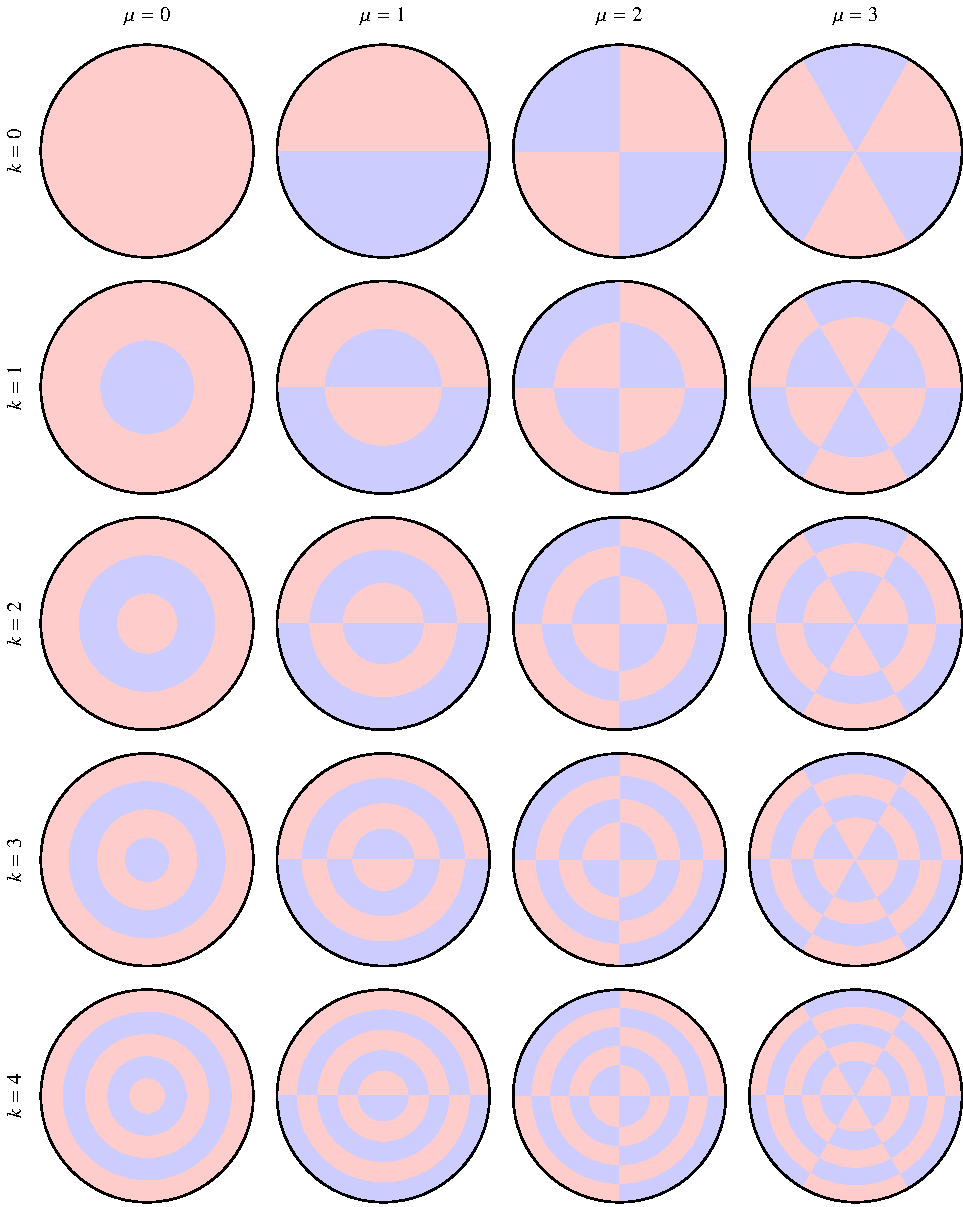
\includegraphics{chapters/090-pde/bessel/pauke.pdf}
\caption{Vorzeichen der Lösungsfunktionen und Knotenlinien
für verschiedene Werte von $\mu$ und $k$.
Die Bereiche, in denen die Lösungsfunktion positiv sind, ist 
rot dargestellt, die negativen Bereiche blau.
In jeder Darstellung gibt es genau $k+\mu$ Knotenlinien.
Die Radien der kreisförmigen Knotenlinien müssen aus den Nullstellen
der Besselfunktionen berechnet werden.
\label{buch:pde:kreis:fig:pauke}}
\end{figure}
